\documentclass[20_original-paper.tex]{subfiles}
\begin{document}

The authors calculate their proposed metrics for a range of relevant MDS corpora and systems.
Their main finding is a high influence of the corpus used on the performance of a given system.

For corpora, the authors highlight differences between datasets that were quantified by their metrics.
They also discern trends over time and between crowd-sourced and non crowd-sourced datasets.

Three of the five corpora analyzed in the paper consist of news articles,  which make up a lot of (particularly early, i.e. early 2000) MDS corpora.
This prominence can be explained by the availability of news articles as well as the value of the real world use case of combining and summarizing news articles.

This explains the papers focus on layout bias, i.e. the influence a tokens position in the document has on the likelihood of making it into the summary.
Layout Bias can be especially prominent in news articles, since reporters aim to provide readers with an overview of the topic within the first few sentences.
This leads to a higher amount of  information relevant to the summary in these early sentences.
The authors show empirically that layout bias present in a corpus carries over to trained models, i.e. that the system will then be more likely to include information from earlier sentences,
even when the input does not show the same layout bias as the training material.\cite{dey-etal-2020-corpora}

A further key observation from the paper is that abstractness in the training corpus is correlated with the abstractness of system generated content.

The influence of corpus on systems can be seen in \ref{results}, which ranks system performance as measured by ROUGE-1/ROUGE-2/F1 Score respectively for every corpus under consideration.
On each dataset, a different MDS system performed best, as denoted by rank 1 and highlighted by the blue color.


\begin{figure}
    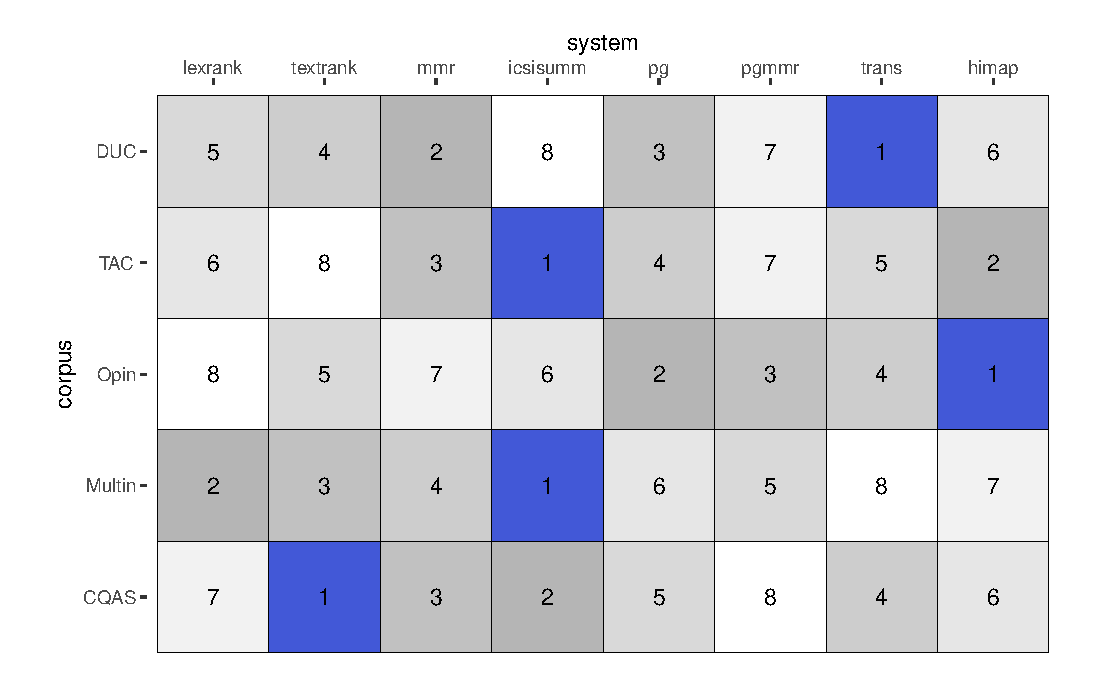
\includegraphics[width=\textwidth]{figures/results.eps}
    \caption{Overview based on the results from the initial paper, where for every MDS system performance over each dataset is ranked and the best performing system for every dataset is highlighted. Lower number indicates better score.} \label{results}
\end{figure}


For ROUGE-1, the only outlier is ICSI\_Summ, which managed to be the  best-performing system on two separate corpora, but also achieved the worst scores on the DUC corpus and the third-worst on Opin.
This indicates the reliance on specific datasets, as opposed to high performance independent of input.\cite{dey-etal-2020-corpora}

The other collected metrics performance metrics, such as ROUGE-2 or F1 Score, do not show the exact same, but still fundamentally similar patterns.
When using F1 to judge quality of generated summaries, for example, there are two systems that achieve the highest score on two separate Corpora instead of just one.
The main observation, that no system strictly outperforms all others, still holds.

Therefore, to make reliable statements about the capabilities of a MDS system,
it is not sufficient to just choose one dataset and report ROUGE scores for that.
Instead, performance over multiple datasets should be considered and reported.

\end{document}